%! BibTeX Compiler = biber
%TC:ignore
\documentclass{article}

\usepackage{xcolor, colortbl}
\definecolor{BLUELINK}{HTML}{0645AD}
\definecolor{DARKBLUELINK}{HTML}{0B0080}
\PassOptionsToPackage{hyphens}{url}
\usepackage[colorlinks=false]{hyperref}
% for linking between references, figures, TOC, etc in the pdf document
\hypersetup{colorlinks,
    linkcolor=DARKBLUELINK,
    anchorcolor=DARKBLUELINK,
    citecolor=DARKBLUELINK,
    filecolor=DARKBLUELINK,
    menucolor=DARKBLUELINK,
    urlcolor=BLUELINK
} % Color citation links in purple
\PassOptionsToPackage{unicode}{hyperref}
\PassOptionsToPackage{naturalnames}{hyperref}

\usepackage{biorxiv}
\usepackage[backend=biber,style=nature]{biblatex}
\addbibresource{codon_models.bib}

\usepackage{url}
\usepackage{amssymb,amsfonts,amsmath,amsthm,mathtools}
\usepackage{lmodern}
\usepackage{xfrac, nicefrac}
\usepackage{bm}
\usepackage{listings, enumerate, enumitem}
\usepackage[export]{adjustbox}
\usepackage{graphicx}
\usepackage{bbold}
\usepackage{pdfpages}
\pdfinclusioncopyfonts=1
\usepackage{lineno}

\newcommand{\UniDimArray}[1]{\bm{#1}}
\newcommand{\BiDimArray}[1]{\bm{#1}}
\DeclareMathOperator{\E}{\mathbb{E}}
\DeclareMathOperator{\Var}{\mathrm{Var}}
\newcommand{\der}{\mathrm{d}}
\newcommand{\e}{\mathrm{e}}
\newcommand{\avg}[1]{\left< #1 \right>} % for average
\newcommand{\Ne}{N_{\mathrm{e}}}
\newcommand{\proba}{\mathbb{P}}
\newcommand{\pfix}{\proba_{\mathrm{fix}}}

\newcommand{\Sphy}{S}
\newcommand{\SphyMean}{\overline{\Sphy}}
\newcommand{\divStrongDel}{\Sphy < -3}
\newcommand{\divDel}{-3 < \Sphy < -1}
\newcommand{\divWeakDel}{-1 < \Sphy < 0}
\newcommand{\divWeakAdv}{0 < \Sphy < 1}
\newcommand{\divAdv}{ \Sphy > 1}
\newcommand{\PdivStrongDel}{\proba \left[ \divStrongDel \right]}
\newcommand{\PdivDel}{\proba \left[ \divDel \right]}
\newcommand{\PdivWeakDel}{\proba \left[ \divWeakDel \right]}
\newcommand{\PdivWeakAdv}{\proba \left[ \divWeakAdv \right]}
\newcommand{\PdivAdv}{\proba \left[ \divAdv \right]}

\newcommand{\Spop}{\beta}
\newcommand{\SpopMean}{\overline{\Spop}}
\newcommand{\polyDel}{\Spop < -1}
\newcommand{\polyNeutral}{-1 < \Spop < 1}
\newcommand{\polyAdv}{ \Spop > 1}
\newcommand{\PpolyDel}{\proba \left[ \polyDel \right]}
\newcommand{\PpolyNeutral}{\proba \left[ \polyNeutral \right]}
\newcommand{\PpolyAdv}{\proba \left[ \polyAdv \right]}

\renewcommand{\baselinestretch}{1.5}
\linenumbers

\title{Empirical evidence for positive selection that is not adaptive evolution}

\author{
    \large
    \textbf{T. {Latrille}$^{1}$, J. {Joseph}$^{2}$, N. {Salamin}$^{1}$}\\
    \normalsize
    $^{1}$Université de Lausanne, Lausanne, Switzerland\\
    $^{1}$Université de Lyon, Lyon, France \\
    \texttt{\href{mailto:thibault.latrille@ens-lyon.org}{thibault.latrille@ens-lyon.org}} \\
}

\begin{document}
    \maketitle

    \begin{abstract}
        Evidence for positive selection occurring in protein-coding DNA sequence is widespread across different taxa.
        Positive selection can be a result of adaptive evolution, meaning that individuals have had to adapt to a change in environment or selective pressure.
        However, current positive selection can also be the result of mutations compensating for deleterious substitutions that have accumulated along lineages, in which case positive selection is non-adaptive and predictable.
        To evaluate the extent of non-adaptive positive selection, we have combined population genetics and phylogenetic datasets.
        We first leveraged phylogenetic codon models which are based on a population-genetics formalism, assuming a non-adaptive fitness landscape.
        These models estimate the fitness of each of the 20 amino acids for each protein site, given mammalian protein-coding DNA alignments and gene tree topologies.
        Second, we integrated mammalian divergence data with polymorphic variants found in 29 populations across 7 mammalian genera.
        For each non-synonymous variant observed at the population level, we predicted its change in fitness from amino-acid fitness estimated at the mammalian scale.
        We found that a large proportion of observed non-synonymous changes are predicted to be positively selected, meaning that the ancestral allele is suboptimal.
        These supposedly advantageous variants are indeed showing signs of recent positive selection in all populations.
        Our work confirms that deleterious substitutions have accumulated across the phylogeny and are currently being compensated for, resulting in widespread positive selection that is not adaptive evolution.
        This study also shows the leverage obtained by integrating phylogenetic and population genetics on a common formalism.
    \end{abstract}

    \keywords{Selection \and phylogenetic \and population genetics \and codon models}

    We usually say that a mutation is undergoing positive selection when it brings a fitness advantage to its bearer, and thus facilitate its own transmission to the next generation.
    However, the causes of this advantage can be diverse.
    We can distinguish two main advantages.
    The first advantage allows its bearer to become better adapted to a new or a changing environment, what we typically call adaptive evolution.
    The population as a whole is thus climbing the fitness landscape along an adaptive walk\cite{tenaillon_utility_2014}.
    The second is non-adaptive, in the sense that the increase in fitness of a new mutation is not a response to a new or a changing environment.
    Instead, the mutation restores the ancestral state which corresponded to an optimal functioning of the individual in a constant environment, but has been lost due to the fixation of a deleterious mutation by drift.
    The population as a whole is thus merely staying in the same position in fitness landscape at this equilibrium, and positive selection compensates for deleterious mutations that reach fixation due to drift\cite{sella_application_2005, mustonen_fitness_2009}.
    These two different kinds of selection result in a positive transmission bias of the advantageous allele, but their consequences are conceptually different.
    While adaptive evolution promotes phenotype diversification, non-adaptive positive selection promotes phenotype stability and preserves well established biological systems.
    It is thus of importance to be able to distinguish those two kinds of positive selection in order to understand the diversification of species.

    Inside proteins, positive selection can be quantified by comparing sequence variation inside a population with the sequence divergence with a sister species\cite{mcdonald_adaptative_1991}.
    Indeed, strongly advantageous mutations are expected to be observed in substitutions but not in polymorphism because they reach fixation quickly.
    This method has been largely improved to account for possible bias-inducing factors such as the presence of weak positive selection, background selection and demography fluctuations\cite{eyre-walker_distribution_2006, eyre-walker_estimating_2009, galtier_adaptive_2016, tataru_inference_2017}.
    It's application across many taxa has uncovered that a large proportion of substitutions are positively selected\cite{moutinho_variation_2019}.
    The root cause for this widespread rate of positive selection is, however, scarcely investigated, often assumed to be the end result of adaptive evolution.
    However, as mentioned above, not all these mutations contribute to genetic innovation and diversification.
    Adaptive evolution can only be well estimated if non-adaptive positive selection is taken into account.
    While adaptive evolution is unpredictable because it brings an advantage concerning an unpredictable change in the environment of organisms, the second is predictable because optimal states should be more or less the same for closely related organisms which share most of their environment and physiology.
    A way to thus measure non-adaptive positive selection is to compute selection coefficients assuming a constant and stable fitness landscape estimated from the alignment of protein-coding genes.
    For each site of the protein alignment, amino-acid frequencies in the alignment is a proxy for its fitness, since for example a deleterious amino acid will be absent in the alignment.
    One of the most used methods to make these predictions is SIFT (Sort Intolerant From Tolerant) which reliably detects deleterious mutations in many taxa\cite{ng_sift_2003, vaser_sift_2016}.
    However, this method has two major shortcomings.
    First, this method uses amino-acid frequency as a proxy for amino-acid fitness, even if we know that a lot of mechanisms can influence amino-acid frequency other than fitness (phylogeny, mutation biases, GC-biased gene conversion, mutational paths).
    Second, each mutation is attributed a score to describe if it should be under purifying selection on one hand or be neutral or advantageous, on the other hand.
    But this score makes little sense to actual measure of fitness, and is not interpretable in terms of population genetics.
    In the other hand, at the DNA level, so-called mutation-selection codon models are rooted with population genetics formalism\cite{halpern_evolutionary_1998, mccandlish_modeling_2014}.
    Such models provide a nearly-neutral framework of evolution by estimating the fitness landscape over amino-acid sequences for each site of the sequence while taking into account non-adaptive processes impacting codon frequency\cite{halpern_evolutionary_1998, rodrigue_mechanistic_2010, tamuri_estimating_2012}.
    Only nearly-neutral mutations between high fitness amino acids will tend to be permitted by the model, allowing for the explicit calculation of the scaled selection coefficient of non-synonymous mutations between codons.
    These models have been used as a null model to predict the overall rate of evolution of proteins\cite{spielman_relationship_2015, dosreis_how_2015}.
    A departure from this model indicates that proteins are evolving under a changing fitness landscape\cite{rodrigue_detecting_2017, tamuri_mutationselection_2021} and is a signal of adaptive evolution\cite{rodrigue_bayesian_2021}.
    In this study we want to address three main questions: which proportions of the polymorphism we observe in mammals is undergoing non-adaptive positive selection ?
    Are these mutations actually under positive selection at the scale of populations ?
    How does effective population size modulates positive, negative and weak selection ?

    \begin{figure*}[!ht]
        \
        \centering
        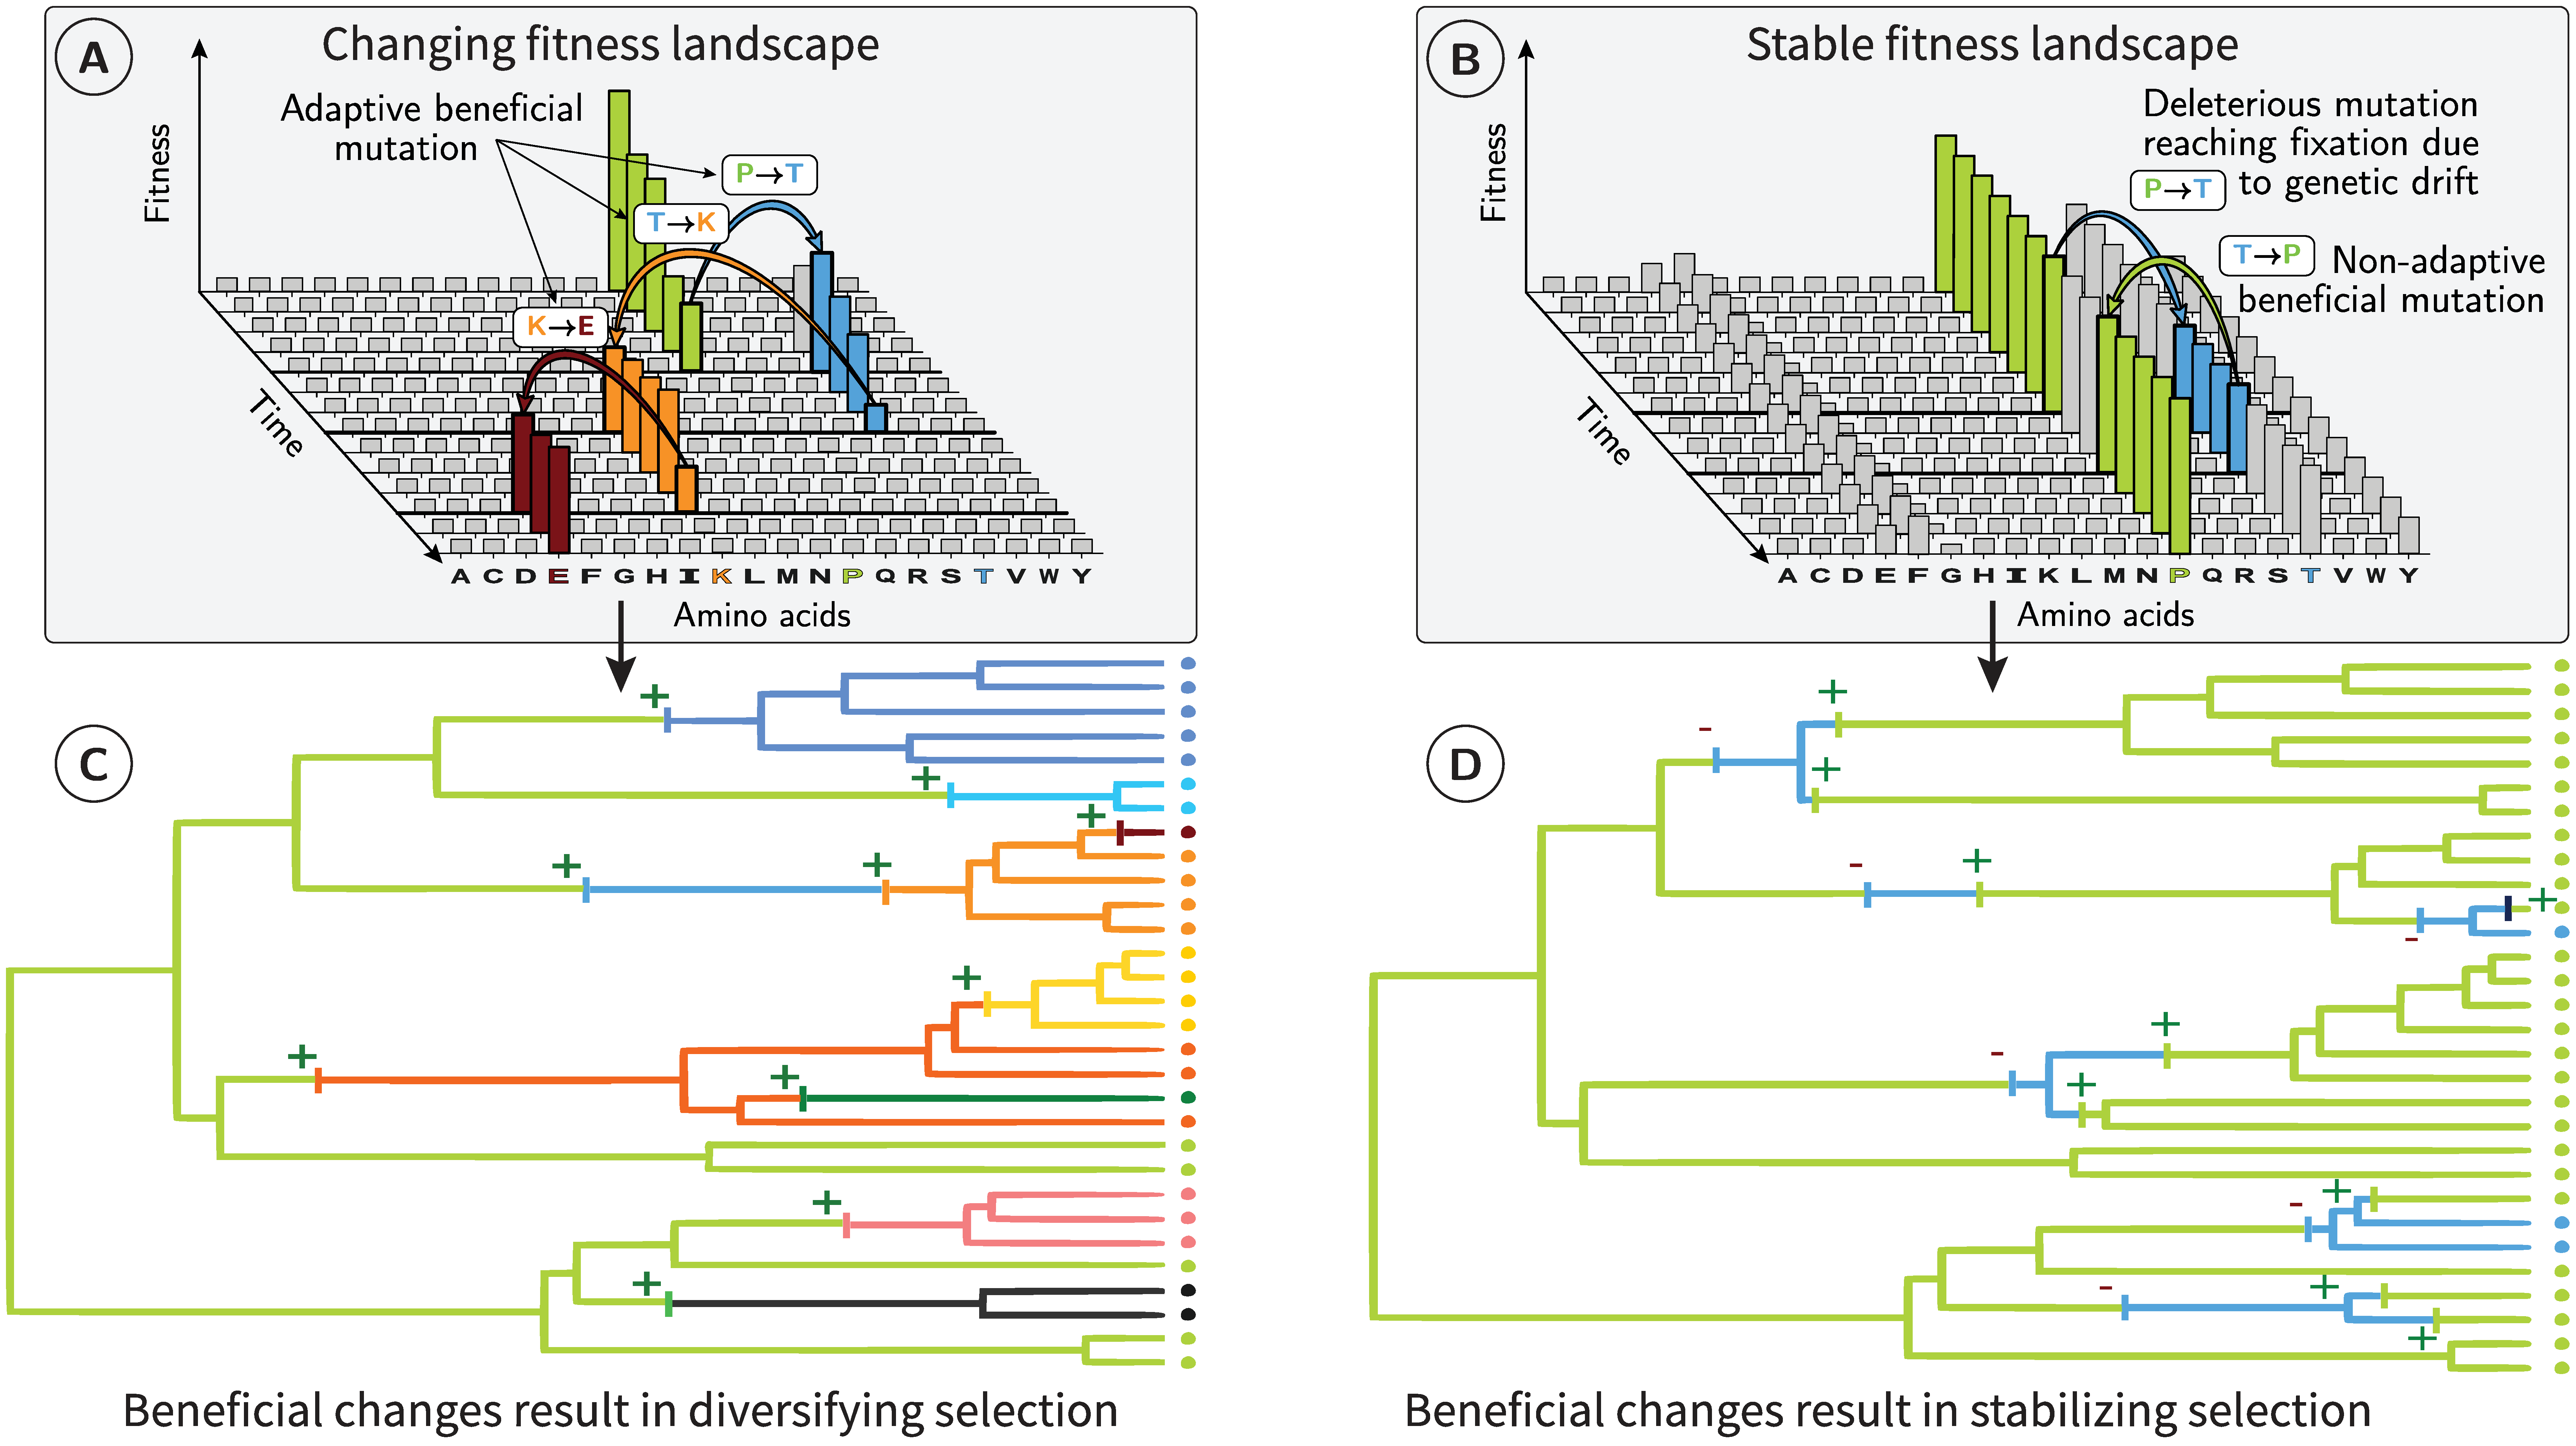
\includegraphics[width=\textwidth, page=1] {artworks/figure1}
        \caption{
            Integrating divergence and polymorphism for the detection of adaptation.
            At the phylogenetic level (panel A), amino-acid Wrightian fitness for each site are estimated from protein-coding DNA alignments using mutation-selection codon models.
            At the population-genetic level (panel B), for each observed single nucleotide polymorphism (SNP), selection coefficient are computed as the difference in amino-acid fitness between the ancestral and derived variant.
        }
        \label{fig:method}
    \end{figure*}

    For this we used available multiple sequence alignment between mammalian species\cite{ranwez_orthomam_2007, howe_ensembl_2021} to estimate fitness landscape on long-term evolution.
    We developed and leveraged a pipeline integrating divergence and polymorphism data across the entire exome for 29 populations across 7 genera, namely \textit{Equus}, \textit{Canis}, \textit{Bos}, \textit{Capra}, \textit{Ovis}, \textit{Chlorocebus} and \textit{Homo} (fig.~\ref{fig:method}).
    For each non-synonymous SNP observed at the population level, we predicted its scaled selection coefficient ($\Sphy$) in fitness from amino-acid fitness estimated at the mammalian scale (fig.~\ref{fig:homo-afr-results}A).
    Then we ask whether the variants that are supposedly advantageous are showing signature of short term positive selection.
    In other words, if a variant is found in many mammals but not in ancestral humans, and a mutation in humans is toward the mammalian version, is this mutation advantageous for the individual carrying it?
    At the population level (e.g. in humans with Asian descent in fig.~\ref{fig:homo-afr-results}), we divided all observed SNPs in 5 classes of predicted selection coefficient: severely deleterious with $\divStrongDel$, deleterious with $\divDel$, weakly deleterious with $\divWeakDel$, weakly advantageous with $\divWeakAdv$ and advantageous with $\divAdv$.
    For each class of selection, SNPs are then grouped by the number of derived alleles in the population (fig.~\ref{fig:homo-afr-results}B), generating so called site-frequency spectrum (SFS).
    Compared to synonymous mutations supposedly neutral (black line in fig.~\ref{fig:homo-afr-results}B), mutations predicted to be deleterious (blue and green lines in fig.~\ref{fig:homo-afr-results}B) are underrepresented at high frequency in the population, a signature of ongoing purifying selection.
    Remarkably, SNPs predicted to be advantageous (red line in fig.~\ref{fig:homo-afr-results}B) are over-represented at higher frequency in the population, meaning they are more likely to reach fixation as a consequence of ongoing positive selection.
    However, these observations remain qualitative.
    Thus, we quantified the distribution of selection coefficient for each category of SNPs with the model polyDFE\cite{tataru_inference_2017, tataru_polydfe_2020}.
    The model uses the count of derived allele for each frequency class of the SFS to infer the distribution of fitness effects (DFE) of the region under study.
    For each category of SNPs, it is important to compute the expected number of mutations giving birth to a SNP of that category given a mutational matrix (fig.~\ref{fig:homo-afr-results}C).
    The model uses both the mutational expectation for each category, and the counts of synonymous derived allele as a neutral model, which allow to control for demographic effects, and polarization errors when inferring the ancestral state.
    These populations based models cannot give a specific estimate of $\Spop$ for each SNP, but by gathering information across many SNPs, these models can estimate the proportion of advantageous mutations ($\PpolyAdv$), of nearly-neutral mutations ($\PpolyNeutral$) and of deleterious mutations ($\PpolyDel$) (fig.~\ref{fig:homo-afr-results}D).
    We found that SNPs predicted to be deleterious given their selection coefficient $\Sphy$ across mammals are effectively purged at the population-genetic scale, demonstrating that purifying selection is largely predictable and amino acids with low fitness across mammals are effectively purged away in each population.
    Notably, SNPs predicted to be advantageous given their selection coefficient $\Sphy$ are indeed under positive selection at the population-genetic scale, confirming that there is a local ongoing selection toward amino acids that are restoring the optimally functioning protein.
    In between these two extremes, mutations predicted to be weakly selected (cyan and orange in fig.~\ref{fig:homo-afr-results}) are effectively composed of neutral, positively and negatively selected mutations.

    We replicated such experiment across 29 populations (fig.~\ref{fig:all-pop-results}), and found that mutations predicted to be deleterious are indeed purged at the population-genetic scale (blue and green rows in fig.~\ref{fig:all-pop-results}A).
    However, mutation predicted to be weakly advantageous ($\divWeakAdv$) are composed of a mix of neutral and selected mutations with varying proportions across the different populations (orange row in fig.~\ref{fig:all-pop-results}B).
    Similarly, mutations predicted to be advantageous are found to be positively selected with varying proportions (red row in fig.~\ref{fig:all-pop-results}C).
    A variable which could explain those variations between populations is the effective number of individuals in the population ($\Ne$), a major driver of selection efficacy.
    $\Ne$ is not directly accessible, and a reasonable proxy usually used is the synonymous diversity ($\theta=4\Ne\mu$ with $\mu$ the mutation rate).
    We thus ordered populations by increased synonymous diversity (fig.~\ref{fig:selcoeff-pop-phylo}A), exhibiting a decreased proportion of neutral mutations.
    This result suggest that populations with higher diversity (e.g.~\textit{Bos} or \textit{Ovis}) are more likely to discriminate whether mutations are advantageous or deleterious.
    Alternatively stated, mutations in populations with low diversity (e.g.~\textit{Homo}) are effectively nearly-neutral and behave as would a neutral mutation.
    This result is qualitatively in accordance with the nearly-neutral theory of evolution that mutations are less efficiently selected for small populations.
    Moreover, we found this effect to be in the same direction but less pronounced when we focused on all SNPs (fig.~S1) rather than only the SNPs predicted to be weakly selected (fig.~S2-3).
    To look further into the relation between diversity and selection efficacy, we thus studied the estimation of the mean $\SpopMean$ as a function of the mean $\SphyMean$ for a subset of SNPs, for which $\SphyMean$ is close to $0$.
    Indeed, polyDFE is a nearly neutral model and is not able to reliably compute selection coefficients for only strongly deleterious or only strongly advantageous SNPs.
    Sliding window of groups of $5.000$ SNPs are taken with a mean $\SphyMean$ between $-0.5$ and $0.5$ (fig.~\ref{fig:selcoeff-pop-phylo}B).
    $\SpopMean$ is estimated for each group, with some groups that might have part of same SNPs that overlap.
    The relationship between $\SpopMean$ and $\SphyMean$ is described as a second-order polynomial, and the slope of this polynomial at $\SphyMean=0$ gives the ratio $\SpopMean/\SphyMean$ for each population.
    We observe that $\SpopMean/\SphyMean$, representing the efficacy of selection at the short versus long-term is positively correlated with synonymous diversity (fig.~\ref{fig:selcoeff-pop-phylo}C), a proxy of effective population size.
    Altogether, populations with large effective population size are under more efficient selection, confirming the prediction of the nearly-neutral theory of evolution.

    As a consequence of increased selection efficacy, mutations in populations with high diversity are mechanically more likely to be deleterious (fig.~S4), especially for mutations predicted already to be deleterious at the phylogenetic scale (fig.~S5-6).
    However, and surprisingly, a decrease in the proportion of neutral mutation did not translate into a mechanical increase in the proportion of advantageous mutations.
    Instead, populations with higher diversity have a lower proportion of advantageous mutations (fig.~S7), this effect is also more pronounced for mutations predicted to be advantageous at the phylogenetic scale (red row in fig.~\ref{fig:all-pop-results}C and fig.~S8).
    This discrepancy can be explained by the fact that populations with larger diversity have already depleted the putatively advantageous mutations, and that only deleterious are remaining possible.
    In other words, being on the top of a fixed fitness landscape leaves you with only paths going downhill.
    Altogether, populations with increased diversity are showing signature of increased selection efficiency and are also less likely to generate positively selected mutations.


    \begin{figure*}[!ht]
        \centering
        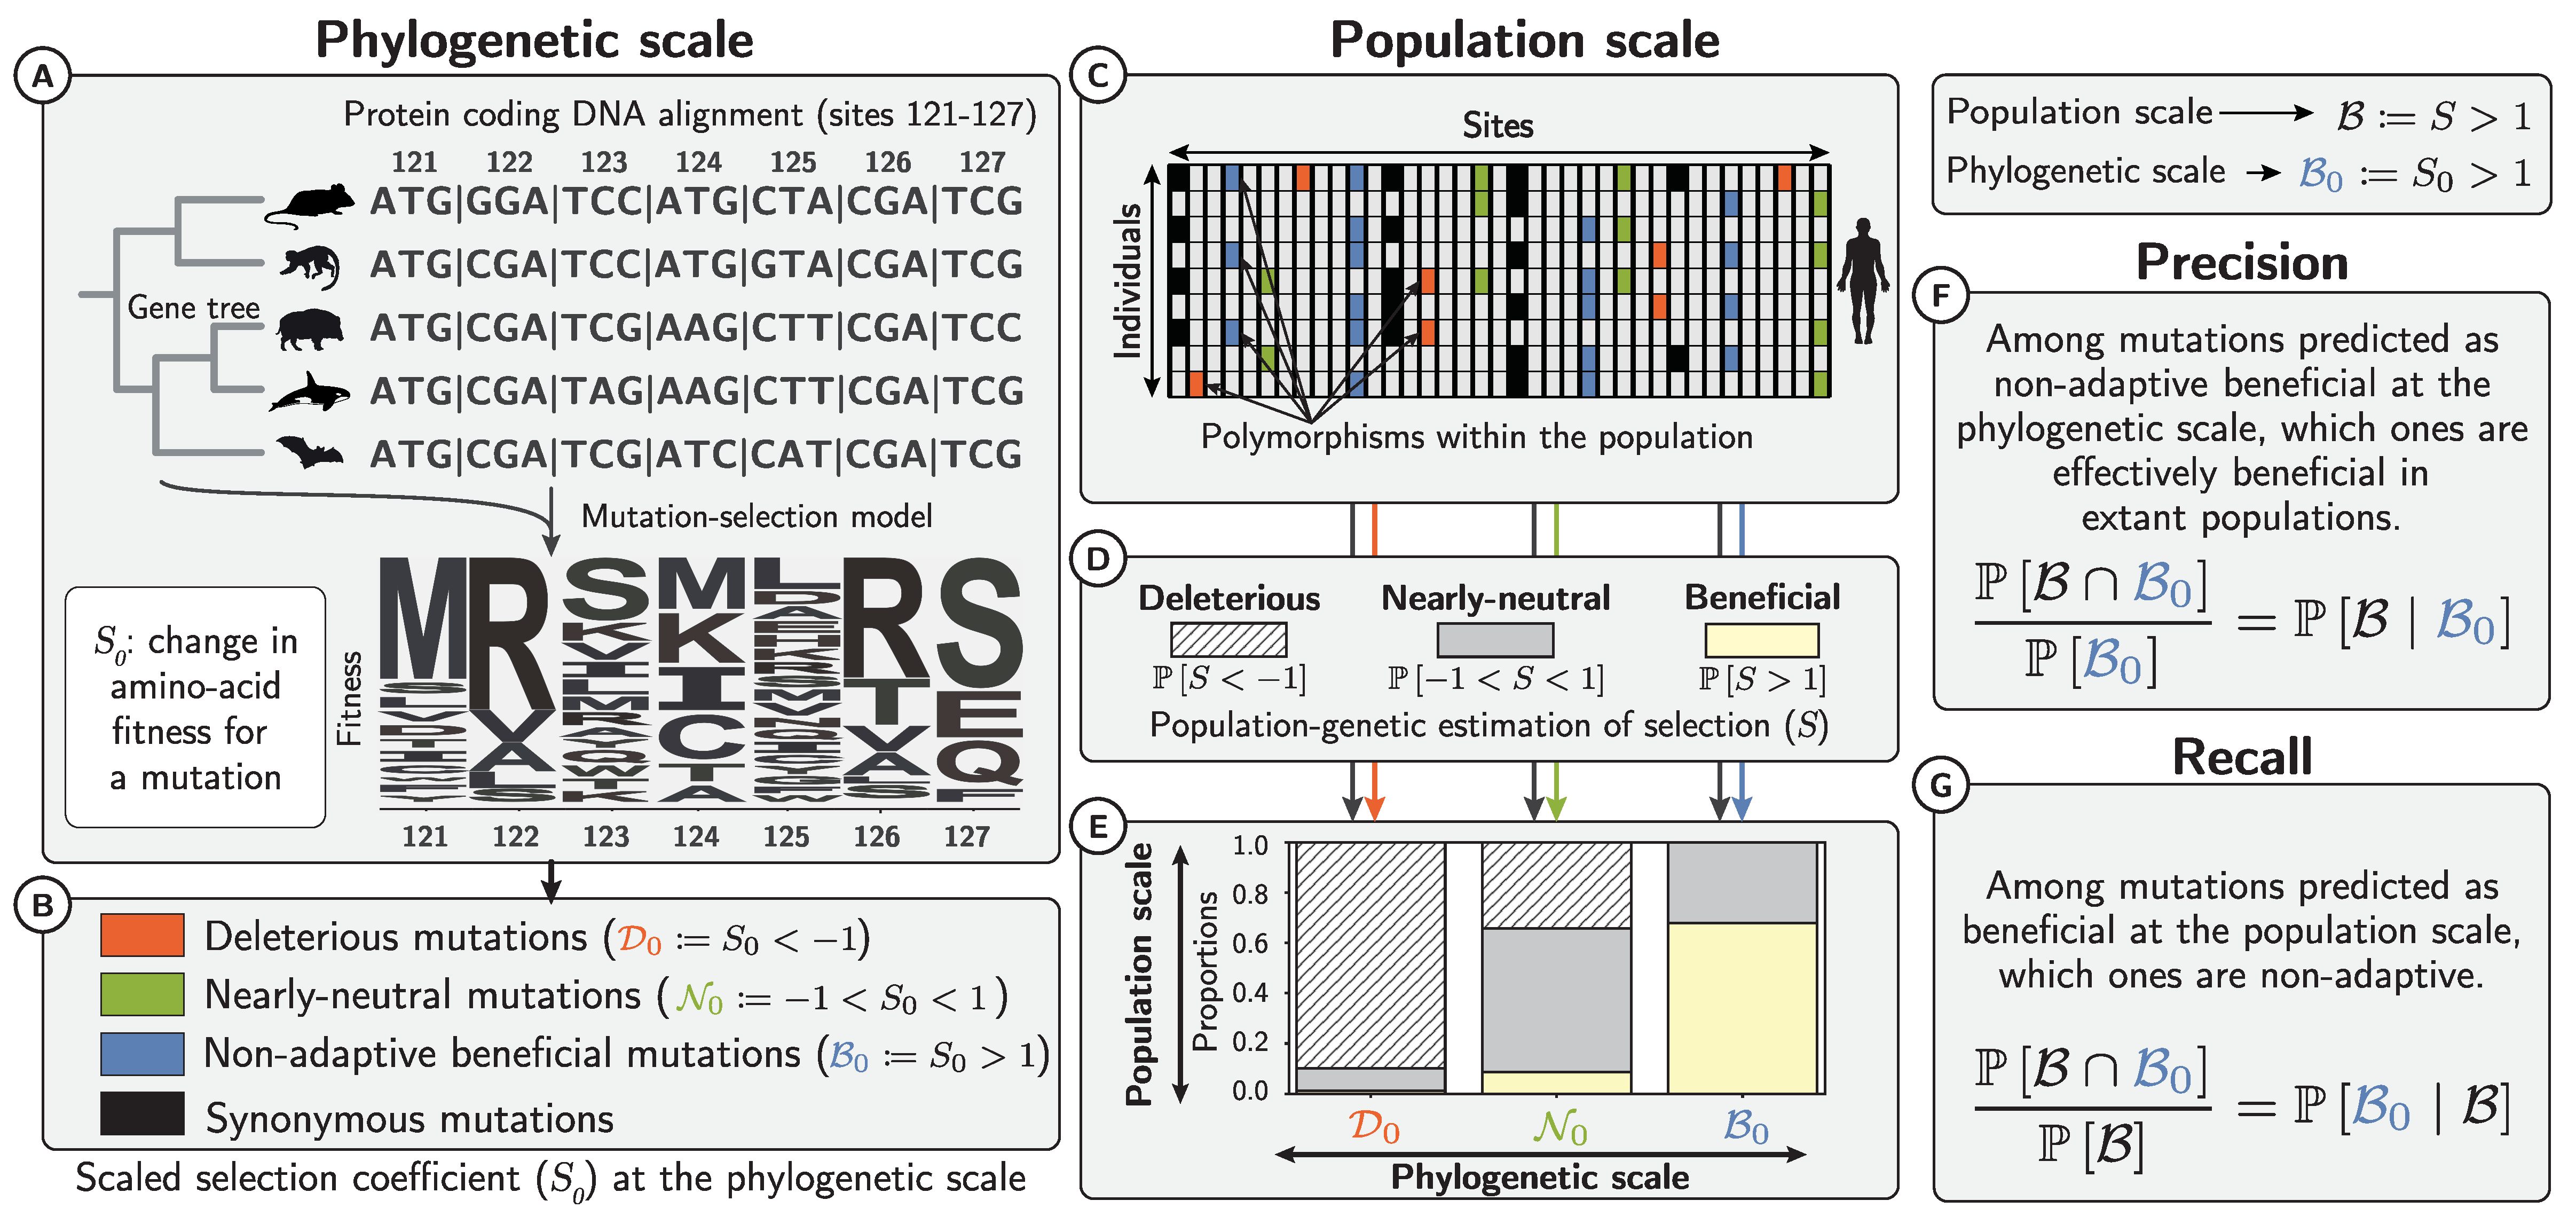
\includegraphics[width=\textwidth, page=1] {artworks/figure2}
        \caption{
            Panel A: Histogram of predicted selection coefficient ($\Sphy$) for each observed mutation in a sample of 8 individuals (out of 512 in the original dataset) with African descent.
            Mutations are divided in 5 classes of selection: severely deleterious (blue), deleterious (green), weakly deleterious (light green), weakly advantageous (yellow) and advantageous (red).
            Panel B: Site-frequency spectrum (SFS) represents the proportion of mutations (y-axis) with a given number of derived alleles in the population (x-axis).
            SFS are drawn for a random sample of 16 alleles (mean in solid line and standard deviation in filled color) for each class of selection and for synonymous mutations supposedly neutral (black).
            Supposedly advantageous are over-represented at higher frequency, while severally deleterious are underrepresented at high frequency, a signature of selection.
            Panel C. Histogram of predicted selection coefficient ($\Sphy$) for each possible mutation away from the ancestral human genome, weighted by the mutation rate.
            For each class of selection, the sum of histogram in this class thus gives the expected total mutation rate toward this class.
            If they are less mutations observed than expected, this class is thus undergoing purifying selection.
            Panel D. For each class of selection (and for the set of all non-synonymous mutations), information from the SFS and the expected total mutation rate are combined at the population-genetic scale to estimate the proportion of advantageous mutations $\PpolyAdv$, of nearly-neutral mutations $\PpolyNeutral$ and of deleterious mutations $\PpolyDel$.
        }
        \label{fig:homo-afr-results}
    \end{figure*}

    \begin{figure*}[!ht]
        \centering
        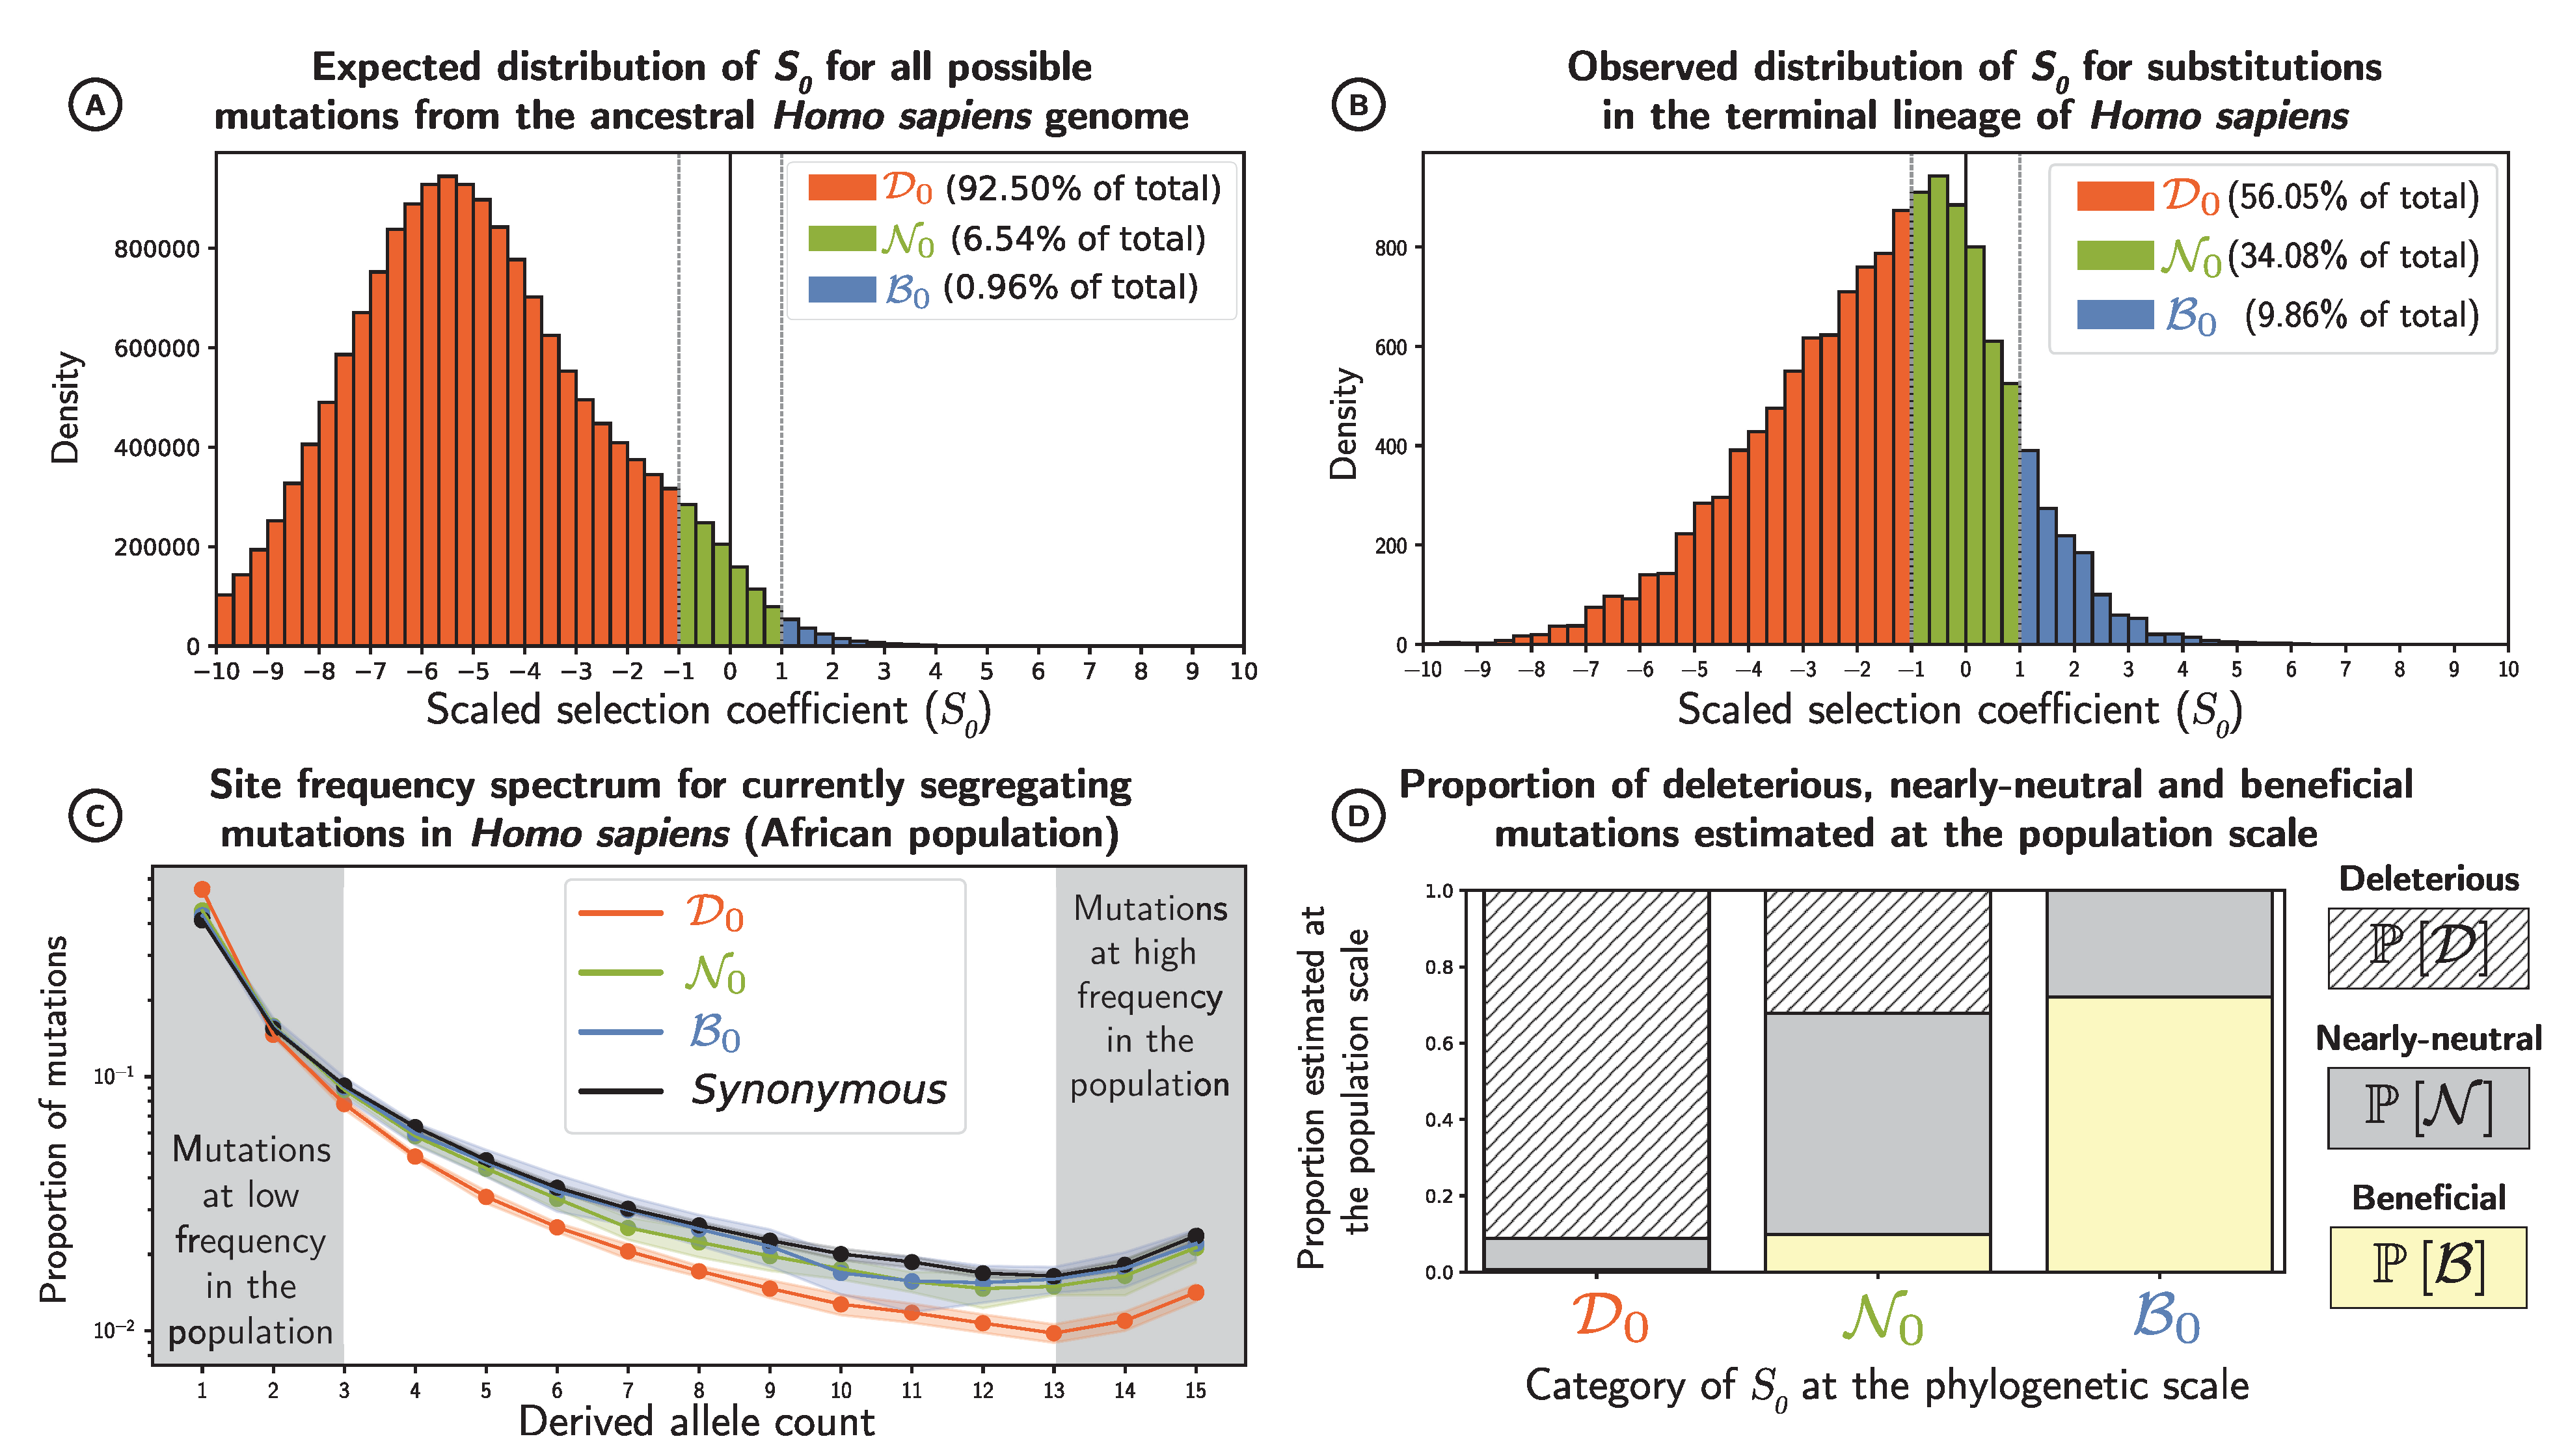
\includegraphics[width=\textwidth, page=1] {artworks/figure3}
        \caption{
            Reproducibility of results shown in figure~\ref{fig:homo-afr-results} in 29 populations across 7 genera.
            Site-frequency spectra and total mutation rates are combined at the population-genetic scale to estimate the proportion of advantageous mutations ($\PpolyAdv$) in top panel, of nearly-neutral mutations ($\PpolyNeutral$) in middle panel and of deleterious mutations ($\PpolyDel$) in bottom panel.
        }
        \label{fig:all-pop-results}
    \end{figure*}

    \begin{figure*}[!ht]
        \centering
        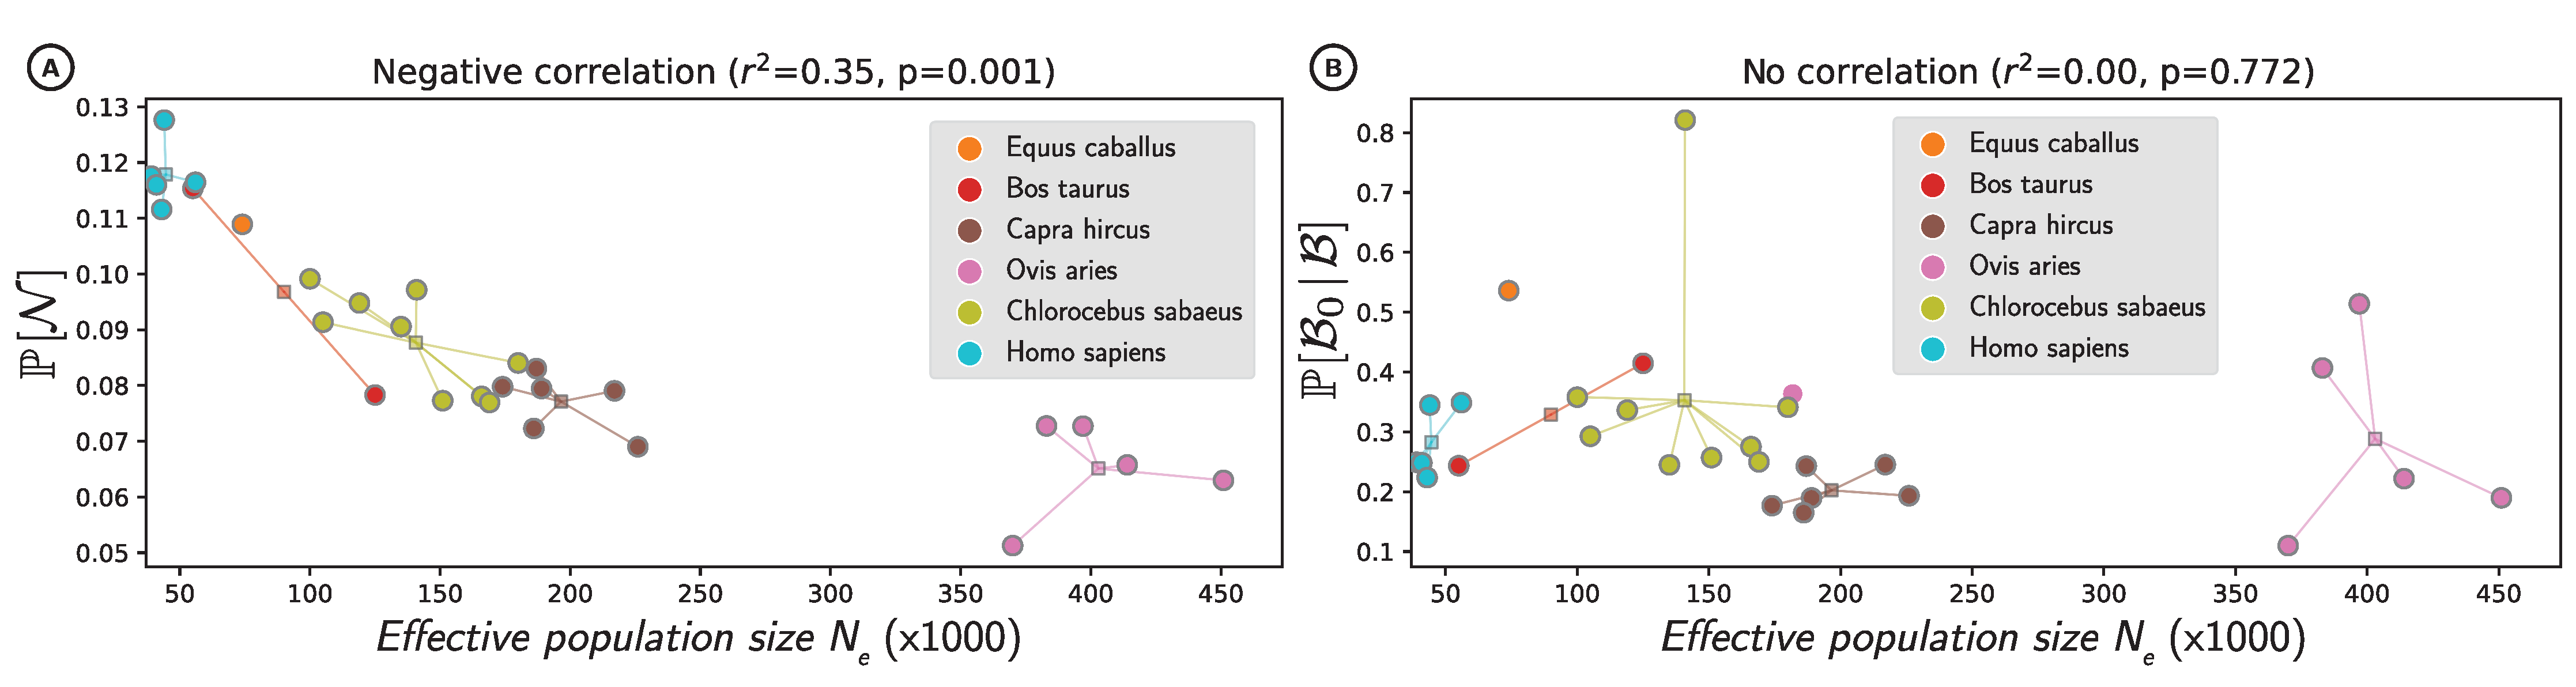
\includegraphics[width=\textwidth, page=1] {artworks/figure4}
        \caption{
            Panel A. For each population, proportion of advantageous ($\PpolyAdv$), nearly-neutral ($\PpolyNeutral$) and of deleterious ($\PpolyDel$) mutations estimated at the population-genetic scale.
            Estimation is performed with SNPs predicted to be weakly advantageous at the phylogenetic scale ($\divWeakAdv$).
            Panel B. Mean selection coefficient at the population scale $\SpopMean$ as a function of phylogenetic $\SphyMean$.
            Observed SNPs are sorted and groups of $5.000$ SNPs are taken as a sliding window with increasing mean $-0.5 \leq \SphyMean \leq 0.5$.
            For each group along the sliding window, $\SpopMean$ (y-axis) is estimated based on SFS and the total mutation rate, and compared to the mean $\SphyMean$ (x-axis).
            A second order polynomial is fitted for each population, and the slope of this polynomial at $\SphyMean=0$ gives the ratio $\SpopMean/\SphyMean$ given in legend.
            Panel C. Ratio $\SpopMean/\SphyMean$ as a function of the synonymous diversity for each population.
            Populations with higher diversity are showing higher ratio of ratio $\SpopMean/\SphyMean$.
        }
        \label{fig:selcoeff-pop-phylo}
    \end{figure*}

    From a structural biology perspective, we found that proteins are not optimal, with a large proportion of mutations still toward more optimal amino acids.
    Seen from another angle, it means that we could theoretically derive the fittest proteins using only the amino acid with the highest fitness.
    Another way to confirm our predictions on amino acid fitness would be to test whether fittest proteins are also thermodynamically more stable, leveraging recent developments able to compute efficiently and accurately the folding of proteins.

    % Our study is a bridge between phylogenetic and population genetics
    From a theoretical evolution perspective, we found that we could use phylogenetic signal to predict the selection coefficient of a mutation.
    Apart from phylogenetic mutation-selection codon models, SIFT scores based on amino-acid alignments across species have already been found to be informative of the selection pressure exerted at the population scale\cite{chen_hunting_2021}.
    Our study concur in that direction, that sites with higher SIFT score at the phylogenetic scale are more positively selected in the different populations (supp.\ mat\  section 2).
    In practice, SIFT score are more coarse grained, with for example a bulk a mutations with a score of 1.0 (the highest), and does not provide a boundary between advantageous and deleterious mutations.
    Moreover, they are not based on population-genetics formalism, hence the relationship between selection coefficient and SIFT score is not straightforward.
    Alternatively at the DNA level, $\omega$-based codon model use the ratio of non-synonymous over synonymous substitution as signature of selection\cite{goldman_codonbased_1994, yang_codonsubstitution_2002}, taking into account the mutational bias and the underlying phylogeny.
    We also show that sites with higher $\omega$ are more positively selected in the different populations (supp.\ mat\  section 3).
    However, even sites which are supposedly under pervasive positive selection at the phylogenetic scale ($\omega>1$) are not necessarily positively selected in the populations.
    Most importantly, such models do not leverage the information of the source and target amino acid involve in the mutation, and thus cannot be used to estimate the non-adaptive part of positive selection.
    Altogether, we showed that mutation-selection codon models formalize a bridge between phylogenetics and population genetics models, but both ends has its limitation and could be improved.

    % Problem with the current mutation-selection model, and the way forward
    Phylogenetic codon models make two assumptions which have a negative impact on the prediction of the selection coefficient.
    First, they are assuming no changes in effective population size while it has been established that population size has a major effect on selection dynamics\cite{lanfear_population_2014, platt_protein_2018}.
    Estimating effective population size along with fitness landscape is possible\cite{latrille_inferring_2021}, but is for the moment too computational intensive to be performed genome-wide\cite{latrille_inferring_2021}.
    Hybrid mutation-selection and $\omega$-based codon model could provide a way forward\cite{brevet_reconstructing_2021}.
    Second, epistasis is not modeled while it can have drastic consequences on the change in fitness landscape\cite{latrille_quantifying_2021}.
    Some models using Direct Coupling Analysis (DCA) can infer coevolution between sites, and thus provide a score of fitness of an amino-acid which depends on other sites of the sequence\cite{bisardi_modeling_2022}.
    However, as SIFT scores, the scores given by DCA are not formalized in terms of selection coefficient and thus are hard to interpret in terms of population genetics, while also neglecting the underlying phylogeny and mutational biases.
    Relaxing both assumptions are computationally intensive\cite{rodrigue_site_2005, kleinman_statistical_2010,latrille_inferring_2021}, and would require new mutation-selection models and optimization techniques to be able to manipulate genome-wide datasets.
    In the other hand, in population-genetic codon models, there is no consensus on the expected shape of the DFE\cite{welch_divergence_2008, bataillon_effects_2014}, but it has indeed be found to be reliably constant between species\cite{castellano_comparison_2019}.
    The model we used allows the inference of a full DFE (both positive and negative), but it has chosen to model the negative part of the DFE as a gamma distribution, and as an exponential one for the positive part.
    However, when we aggregate SNPs that are expected to be strongly deleterious or strongly advantageous, the model struggles to fit their DFE to a gamma or an exponential distribution.
    As a result, while the proportions of negative/weak/positive mutations stays reliable, the mean values for selection coefficients ($\Spop$) estimated by polyDFE become biologically absurd ($\Spop \ll -10^3$).
    Such effect is not found for neutral SNPs and to method to accurately estimate the mean value of selection coefficients from SFS without assuming any shape for the DFE remains yet to be available.

    Aside from methodological limitations, the mammalian case study might also not be representative of other clades.
    Indeed, our dataset is quite convenient because of relatively small population sizes since a large amount of deleterious mutations are fixed, and thus, there is a lot of opportunities for non-adaptive positive selection to arise.
    It would thus be of great interest to reproduce our experiment with other clades, such as \textit{drosophila} or birds which have higher effective population size.
    It would also be interesting to have access to more shallow but wider phylogenies to increase the resolution of our predictions.
    % Moreover, mammalian are less affected by codon usage


    \section*{Acknowledgment}
    \label{sec:acknowledgment}
    We gratefully acknowledge the help of Nicolas Lartillot for his advice and review concerning this manuscript.
    This work was performed using the computing facilities of the CC LBBE/PRABI\@.
    \textbf{Funding:}
    Université de Lausanne;
    French National Research Agency, Grant ANR-19-CE12-0019 / HotRec.
    \textbf{Author contributions:}
    Original idea: T.L.\ and J.J.;
    Model conception: T.L., J.J.\ and N.S.;
    Code: T.L.;
    Data analyses: T.L.\ and J.J.;
    Interpretation: T.L., J.J.\ and N.S.;
    First draft, editing and revisions: T.L., J.J.\ and N.S.;
    Project management and funding: N.S\@.
    \textbf{Competing interests:}
    The authors declare no conflicts of interest.
    \textbf{Data and materials availability:}
    Snakemake pipeline, analysis scripts and documentation are available at \href{https://github.com/ThibaultLatrille/SelCoeff}{github.com/ThibaultLatrille/SelCoeff}.


    \section{Material \& Methods}
    \label{sec:methods}

    \subsection{Phylogenetic dataset}

    Protein-coding DNA sequences alignments in placental mammals are extracted from the \href{https://www.orthomam.univ-montp2.fr}{OrthoMaM} database\cite{ranwez_orthomam_2007, douzery_orthomam_2014, scornavacca_orthomam_2019}.
    Genes located on the X, Y and mitochondrial chromosome are discarded from the analysis, since the number of polymorphism, necessary in population-based method, is expected to be different on these sequences.
    Additionally, sequences from the species for which polymorphism are available, as well as their sister species have been discarded from the analysis to ensure independence between the data used in the phylogenetic and population-genetic method.

    \subsection{Selection coefficient ($\Sphy$) in phylogeny-based method}
    \label{subsec:s-phylogeny-method}

    Mutation-selection models assume that the protein-coding sequence is at mutation-selection balance under a fixed fitness landscape, which is itself characterized by a fitness vector over the $20$ amino-acid at each site\cite{yang_mutationselection_2008, halpern_evolutionary_1998, rodrigue_mechanistic_2010}.
    Mathematically, the rate of non-synonymous substitution from codon $a$ to codon $b$ ($q_{a \mapsto b}^{(i)}$) at site $i$ of the sequence is equal to the rate of mutation from the underlying DNA change ($\mu_{a \mapsto b}$) multiplied by the scaled probability of fixation of the mutation ($\proba_{a \mapsto b}^{(i)}$).
    Crucially, the probability of fixation depends on the difference of scaled fitness between the amino-acid encoded by the mutated codon ($F_b^{(i)}$) and the fitness of the amino-acid encoded by the original codon ($F_a^{(i)}$) of site $i$\cite{wright_evolution_1931, fisher_genetical_1930}.
    Altogether, the rate of substitution from codon $a$ to $b$ at a given site $i$ is:
    \begin{equation}
        \begin{dcases}
            q_{a \mapsto b}^{(i)} & = 0 \text{ if codons $a$ and $b$ are more than one mutation away,} \\
            q_{a \mapsto b}^{(i)} & = \mu_{a \mapsto b} \text{ if codons $a$ and $b$ are synonymous,} \\
            q_{a \mapsto b}^{(i)} & = \mu_{a \mapsto b}  \mu_{a \mapsto b} \dfrac{F_b^{(i)} - F_a^{(i)}}{1 - \e^{F_a^{(i)} - F_b^{(i)}}} \text{ if codons $a$ and $b$ are non-synonymous}.
        \end{dcases}
    \end{equation}
    Fitting the mutation-selection model on a sequence alignment leads to an estimation of the mutation rate matrix ($\UniDimArray{\mu}$) as well as the 20 amino-acid fitness landscape ($\UniDimArray{F^{(i)}}$) at each site $i$.
    The selection coefficient for a mutation from codon $a$ to codon $b$ at site $i$ is defined :
    \begin{equation}
        S_{a \mapsto b}^{(i)} = \Delta F^{(i)} = F^{(i)}_{b} - F^{(i)}_{a}.
    \end{equation}
    In the manuscript and the following material, the source ($a$) and target ($b$) codons as well as the site ($i$) are implicit and thus never explicitly written.
    We ran the Bayesian software \href{https://github.com/bayesiancook/bayescode}{BayesCode} on each protein-coding DNA alignment\cite{lartillot_phylobayes_2013, rodrigue_detecting_2017, rodrigue_bayesian_2021}.
    Each Monte-Carlo Markov-Chain (MCMC) is run during $2000$ points, with a burn-in of $1000$ points, allowing to compute the mean amino-acid fitness landscape ($\UniDimArray{F^{(i)}}$) at each site $i$ across the MCMC\@.

    \subsection{Polymorphism dataset}
    \label{subsec:polymorphism-dataset}

    In order to compare polymorphism and divergence, each SNP (chromosome, position, strand) in the focal species must be matched to its relative position in the protein-coding DNA alignment.
    First, genomic positions are converted to relative position in the coding sequence (CDS) using gene annotation files (GTF format) downloaded from Ensembl (\url{ensembl.org}), we verified the SNP match the reference in the CDS (FASTA format) also downloaded from Ensembl.
    Secondly, relative position in the CDS is converted to position in the multiple sequence alignment (containing gaps) from OrthoMaM database\cite{ranwez_orthomam_2007, douzery_orthomam_2014, scornavacca_orthomam_2019} by doing a global pairwise alignment (Biopython pairwise2) between the CDS fasta and the sequence found in the alignment.
    This conversion from genomic position to position in the alignment is only possible if the assembly used for SNP calling is the same as the one used in the alignment, the GTF annotations and the FASTA sequences.
    We retrieved polymorphism from different projects.
    \textit{Equus caballus} variants called on the EquCab2 assembly in the EVA study PRJEB9799.
    \textit{Canis familiars} variants called on the CanFam3.1 assembly in the EVA study PRJEB24066.
    \textit{Bos taurus} variants called on the UMD3.1 assembly in the next-gen project.
    \textit{Ovis aries} variants called on the Oar\_v3.1 assembly in the next-gen project.
    \textit{Capra Hircus} variants called on the CHIR1 assembly in the next-gen project, we performed a liftover to the ARS1 assembly.
    \textit{Chlorocebus sabaeus} variants are called on the ChlSab1.1 assembly in the EVA study PRJEB22989\cite{svardal_ancient_2017}.
    \textit{Homo sapiens} variants are called on the GRCh38 assembly in the 1000-genome project\cite{consortium_integrated_2012, the1000genomesprojectconsortium_global_2015}.
    Variants not inside genes are discarded at the beginning of the analysis.
    Insertions and deletions are not analyzed, and only Single Nucleotide Polymorphisms (SNPs) with only one mutant allele are considered.
    Stop codon mutants are also discarded.
    For populations containing more than $8$ sampled individuals, the site-frequency spectrum (SFS) is subsampled down to $16$ chromosomes ($8$ diploid individuals) without replacement (hyper-geometric distribution) to alleviate the effect of different sampling depth in the $29$ populations.
    SNPs are polarized using the $3$ closest out-groups found in the OrthoMam alignment with est-usfs\cite{keightley_inferring_2018}.
    The Snakemake pipeline for integrating polymorphism and divergence data uses custom scripts written in python 3.9.

    \subsection{Selection coefficient ($\Spop$) in population-based method}
    \label{subsec:s-polymorphism-method}
    The probability to sample allele at a given frequency (before fixation or extinction) is informative of its scaled selection coefficient at the population scale ($\Spop$).
    Pooled across many sites, the SFS is thus informative on the underlying $\Spop$ of mutations, given we have a neutral expectation.
    In this configuration, a single $\Spop$ for all sampled mutations is biologically not realistic.
    Accordingly, a distribution of fitness effects of mutations (DFE) is assumed, usually modeled as a continuous distribution\cite{eyre-walker_distribution_2006, eyre-walker_estimating_2009}.
    In this study, we used the software polyDFE\cite{tataru_inference_2017, tataru_polydfe_2020}, for which the DFE ($\phi$) is given by a mixture of a $\Gamma$ and Exponential distributions, parameterized by $\Spop_d$ , $b$, $p_b$
    and $\Spop_b$ as:
    \begin{equation*}
        \phi \left( \Spop; \Spop_d , b, p_b, \Spop_b \right) =
        \begin{dcases}
            \left( 1 - p_b \right) f_{\Gamma}(-\Spop; -\Spop_d, b) & \text{ if $\Spop \leq 0$,} \\
            p_b f_{e}(\Spop; \Spop_b) & \text{ if $\Spop > 0$,} \\
        \end{dcases}
    \end{equation*}
    where $\Spop_d < 0 $ is the mean of the DFE for $\Spop \leq 0$,
    $b > 0$ is the shape of the $\Gamma$ distribution,
    $0 \leq p_b \leq 1$ is the probability that $\Spop > 0$,
    $\Spop_b > 0$ is the mean of the DFE for $\Spop > 0$,
    and $f_{\Gamma}(x; m, b)$ is the density of the $\Gamma$ distribution with mean m and shape b, while $f_{e}(x; m)$ is the density of the Exponential distribution with mean $m$.
    Once the DFE is fitted to the data, the proportion of advantageous ($\PpolyAdv$), nearly-neutral ($\PpolyNeutral$) and deleterious mutations ($\PpolyDel$) are given as:
    \begin{align*}
        \PpolyAdv &= p_b \int_{1}^{+\infty} f_{e}(\Spop; \Spop_b) \der \Spop  \\
        \PpolyNeutral &= p_b \int_{0}^{1} f_{e}(\Spop; \Spop_b) \der \Spop + \left( 1 - p_b \right) \int_{0}^{1} f_{\Gamma}(\Spop; -\Spop_d, b) \der \Spop \\
        \PpolyDel &= \left( 1 - p_b \right) \int_{1}^{+\infty} f_{\Gamma}(\Spop; -\Spop_d, b) \der \Spop
    \end{align*}
    And finally, the mean of the DFE $\overline{\Spop}$ is given by:
    \begin{align*}
        \SpopMean & = \int_{-\infty}^{+\infty} \Spop \phi \left( \Spop; \Spop_d , b, p_b, \Spop_b \right) \der \Spop \\
        & =  p_b \Spop_b + \left( 1 - p_b \right) \Spop_d
    \end{align*}
    PolyDFE requires one SFS for non-synonymous mutations and one for synonymous mutations (neutral expectation), as well as the total mutation rate (mutation rate per site multiplied by the number of sites) on which each SFS has been sampled.
    The number of sites for each SFS is thus obtained using the following four-step procedure.
    First, for each gene, the reference DNA sequence is adjusted with ancestral and fixed polymorphism for each population.
    Second, from this reconstructed sequence, all possible mutations are computed, weighted by the mutation rate between nucleotide estimated at the phylogenetic scale $\UniDimArray{\mu}$.
    Third, these possible mutations are then classified whether they are synonymous or non-synonymous (stop mutations are excluded), non-synonymous mutations are then also classified depending on their selection coefficient ($\Sphy$).
    Fourth, the number of sites for each class of selection coefficient is then computed as the total number of sites across the genome weighted by the ratio of the aggregated mutations rates falling in the class over the total mutation rate for all possible mutations.
    From the SFS and the number of sites for the both synonymous and for the class of non-synonymous, polyDFE estimates parameters of the DFE $\phi \left( \Spop; \Spop_d , b, p_b, \Spop_b \right)$ using maximum likelihood.

    \printbibliography
\end{document}